\author{Marcin Szymczak}
\title{Badanie Efektu Halla}
\date{3 listopad 2010\\ sroda 9.15}
\documentclass[12pt,a4paper]{article}
\usepackage[latin1]{inputenc}
\usepackage{amsmath}
\usepackage{mathtools}
\usepackage{amsfonts}
\usepackage{amssymb}
\usepackage{graphicx}
\begin{document}
\maketitle
\newpage

\section*{I. Zestaw przyrzadow}
\begin{flushleft}
\begin{itemize}
	\item Elektromagnes EL-01
\item Zasilacz elektromagnesu ZT-980-4
\item Zasilacz hallotronu
\item Woltomierz do pomiaru napiecia Halla
\item Miliamperomierz o maksymalnym zakresie 30 mA do pomiaru natezenia pradu sterujacego
\item Miliamperomierz o minimalnym zakresie 150 mA do pomiaru natezenia pradu plynacego przez
elektromagnes.
\item Hallotron
\item Przystawka hallotronu
\end{itemize}

%-------------------------------------------------------------------WYNIKI POMIAROW ----------------------------
\section*{II. Wyniki pomiarow i obliczen}
\begin{center}



\begin{tabular}{|c|c|c|}
\hline n & I_s [A] & U_H [V]\\ 
\hline 1 & 0.00050 & 0.0008 \\
\hline 2 & 0.00100 & 0.0016 \\ 
\hline 3 & 0.00150 & 0.0025 \\ 
\hline 4 & 0.00200 & 0.0033 \\ 
\hline 5 & 0.00250 & 0.0040 \\ 
\hline 6 & 0.00300 & 0.0049 \\ 
\hline 7 & 0.00350 & 0.0056 \\ 
\hline 8 & 0.00400 & 0.0063 \\ 
\hline 9 & 0.00450 & 0.0072 \\ 
\hline 10 & 0.00500 & 0.0079 \\ 
\hline 11 & 0.00550 & 0.0087 \\ 
\hline 12 & 0.00600 & 0.0094 \\ 
\hline 13 & 0.00650 & 0.0100 \\ 
\hline 14 & 0.00700 & 0.0107 \\ 
\hline 15 & 0.00750 & 0.0114 \\ 
\hline 16 & 0.00800 & 0.0121 \\ 
\hline 17 & 0.00850 & 0.0128 \\ 
\hline 18 & 0.00900 & 0.0134 \\ 
\hline 19 & 0.00950 & 0.0141 \\ 
\hline 20 & 0.01000 & 0.0147 \\ 
\hline
\end{tabular} 
$\displaystyle\forall I_{si}: i \in\{1.. 20\} : \begin{cases} I_m = 130[mA] \\ \Delta I_{si} = 0.08[mA] \\ \Delta I_{mi} = 0.8 [V] \\ 
	\Delta U_{Hi} = 0.0002 [V] \\ B = 440.6 [mT] \\ \Delta B = 2.8 [mT] \end{cases}$ \\

\begin{tabular}{|c|c|c|c|}
\hline n & I_m [A] & U_H [V] & B[T] \\ 
\hline 1 & 0.020 & 0.0201 & 0.0688\\ 
\hline 2 & 0.030 & 0.0308 & 0.1026\\ 
\hline 3 & 0.040 & 0.0462 & 0.1364\\ 
\hline 4 & 0.050 & 0.0564 & 0.1702\\ 
\hline 5 & 0.060 & 0.0660 & 0.2040\\ 
\hline 6 & 0.070 & 0.0742 & 0.2378\\ 
\hline 7 & 0.080 & 0.0829 & 0.2716\\ 
\hline 8 & 0.090 & 0.0942 & 0.3054\\ 
\hline 9 & 0.100 & 0.1015 & 0.3392\\ 
\hline 10 & 0.110 & 0.1126 & 0.3730\\ 
\hline 11 & 0.120 & 0.1188 & 0.4068\\ 
\hline 12 & 0.130 & 0.1304 & 0.4406\\ 
\hline 13 & 0.140 & 0.1372 & 0.4744\\ 
\hline 14 & 0.150 & 0.1442 & 0.5082\\ 
\hline 
\end{tabular} 
$\forall I_{mi} : i \in\{1..20\} : \begin{cases}I_s = 10[mA] \\ \Delta I_{si} = 0.08[mA] \\ \Delta I_{mi} = 0.8[mA]\\ \Delta U_{Hi} = 0.0002 [V]
	\\ \Delta B = 2.8 [mT] \end{cases}$ \\


\end{center}
Klasa przyrzadu, ktorym wykonano pomiary $I_s \wedge I_m$ wynosi 0.5. \\
Pomiar $I_m$ wykonano przy zakresie 150 [mA]. Pomiar $I_s$ wykonano przy zakresie 15 [mA]
\newline

\gamma_1 = 3.32 \pm 0.03[\frac{V}{AT}] \\
\gamma_2 = 28 \pm 0.6[\frac{V}{AT}]
\\

n_1  = 9,41 \cdot 10^{23} \pm  5.65\cdot 10^{22} \left[\displaystyle\frac{1}{m^3}\right] \\
n_2 =  1.12 \cdot 10^{24} \pm 8.06 \cdot 10^{22} \left[\displaystyle\frac{1}{m^3}\right]\\

%------------------------------------------------------------------------------OBLICZENIA -----------------------------
\section*{III. Przykladowe obliczenia}
\noindent
\begin{flushleft}
\(
\Delta I_s \wedge \Delta I_m = \displaystyle\frac{\text{klasa}\cdot \text{zakres}}{100} ; \;\; \text{np. dla } I_m: \\
\Delta I_m = \displaystyle\frac{0.5 \cdot 150}{100} = 0.75 \approx 0.8 [V]\\ 
\)

\

\(
\Delta U_H = 0.05\% \cdot \text{wartosc pomiaru} + 0.01\% \cdot \text{zakres} \;\; \text{np. dla } U_{H14}: \\
\Delta U_{H14} = 0.05\% \cdot 0.1442 + 0.01\% \cdot 1 = 1.721\cdot 10^{-4} [V]
\)

\newpage

\(
\text{B zostalo policzone przy pomocy wzoru podanego w instrukcji roboczej do cwiczenia.} \\
\text{We wszystkich obliczeniach jednostka} I_{mi} \text{ jest [mA]} \\
B = 3.38 \cdot I_{mi} + 1.19 [mT] \;\; \text{np. dla } I_{m1}: \\
B_{1} = 3.38 \cdot 20 + 1.19 = 68.790 [mT]
\)

\

\(
\Delta B  = \left| \displaystyle\frac{\partial B}{\partial I_m} \cdot \Delta I_m\right| = 2.704 \approx  2.8 [mT]

\
\begin{center}
Obliczenia wykonane dla pierwszej tabeli.
\end{center}
%------------------gamma1---------
\gamma \text{ Zostala obliczona przy pomocy regresji liniowej i wynosi }  3.32 [\frac{V}{AT}] \\
\Delta \gamma =  0.03[\frac{V}{AT}] \\
\displaystyle\frac{\Delta \gamma}{\gamma} = \frac{0.03 }{3.32} \approx 0.01

%-------------------n1--------------
n = \displaystyle\frac{1}{e\cdot \gamma \cdot d} = 9.41 \cdot 10^{23}  \left[\displaystyle\frac{1}{m^3}\right] \\
\Delta n = \left(\left| \displaystyle\frac{\Delta d}{d}\right| + \left| \displaystyle\frac{\Delta \gamma}{\gamma}\right|\right)\cdot n = 5.65 \cdot 10^{22} \left[\displaystyle\frac{1}{m^3}\right] \\
\displaystyle\frac{\Delta n}{n} = \frac{5.65 \cdot 10^{22}}{9.41 \cdot 10^{23}} = 0.06

\begin{center}
Obliczenia wykonane dla drugiej tabeli.
\end{center}
%-----------------------gamma2-------------------
\gamma \text{ Zostala obliczona przy pomocy regresji liniowej i wynosi }  28.0 [\frac{V}{AT}] \\
\Delta \gamma = 0.6[\frac{V}{AT}] \\
\displaystyle\frac{\Delta \gamma}{\gamma} = \frac{0.6}{28.0} = 0.022\\

\

%------------------------n2-----------------
n = \displaystyle\frac{1}{e\cdot \gamma \cdot d} = 1.12 \cdot 10^{24} \left[\displaystyle\frac{1}{m^3}\right]\\
\Delta n = \left(\left| \displaystyle\frac{\Delta d}{d}\right| + \left| \displaystyle\frac{\Delta \gamma}{\gamma}\right|\right)\cdot n = 8.06 \cdot 10^{22} \left[\displaystyle\frac{1}{m^3}\right]\\
\displaystyle\frac{\Delta n}{n} = \frac{n = 8.06 \cdot 10^{22}}{1.12 \cdot 10^{24}} = 0.072 

\text{Do obliczen wykorzystano program regresja.exe dostepny na stronie instytutu fizyki,} \\ 
\text{oraz program Octave}
\newpage
%-----------------------------------------------------------------------------WYKRESY----------------------------
\section*{IV. Wykresy}
\begin{center}
Wykresy wykonane dla pierwszej tabeli.
\end{center}
\includegraphics[scale=1]{/home/demoon/UhodI.eps} 
\includegraphics[scale=1]{/home/demoon/gamma2.eps} 
\begin{center}
\newpage
Wykresy wykonane dla drugiej tabeli.
\end{center}
\includegraphics[scale=1]{/home/demoon/UhodB.eps} 
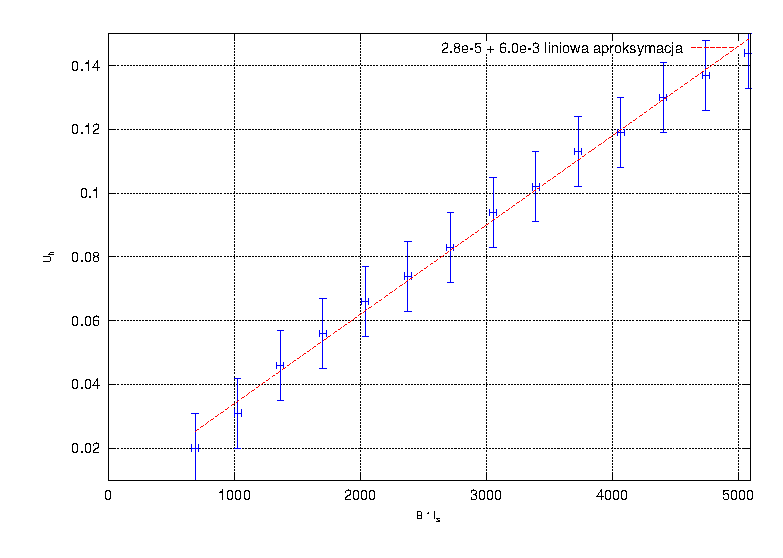
\includegraphics[scale=1]{/home/demoon/gamma.eps} 


%--------------------------------------------------------------------------------WNIOSKI--------------------------
\section*{V. Wnioski}
\begin{itemize}
	\item W protokole nie zapisano jaka najmniejsza dzialke mozna odczytac przy pomocy przyrzadow analogowych. Mozna przypuszczac, ze niepewnosc pomiarowa wynikajaca
		z odczytu bedzie przewyzszac ta obliczona ze wzoru $\frac{\text{klasa} \cdot \text{zakres}}{100}$ .W takim przypadku nalezy zmienic
		$I_m, I_s$ na niepewnosc wynikajaca odczytu z urzadzenia.
\end{itemize}

\end{flushleft}


\end{document}